\section{Layer~12 – Ontological Reconciliation}
\label{sec:layer12}

% ----- SUPERKRACHT -----
\begin{tcolorbox}[colback=blue!5, colframe=blue!60, title=\textbf{Superpower: The Bridge‑Builder}]
\begin{center}
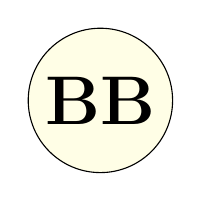
\begin{tikzpicture}
  \node[draw, circle, fill=yellow!10, minimum size=1.5cm, font=\bfseries\Huge] {BB};
\end{tikzpicture}
\textit{“How can two different views be combined?”}
\end{center}
\end{tcolorbox}

Pixel now has two ways of looking at the world: through its camera
and (if we give it a microphone) through sound.  Those two worlds
don’t automatically fit together.  Layer~12 builds a \textbf{bridge}
between such different perspectives.

\begin{tcolorbox}[colback=yellow!5, colframe=yellow!80, title=Real‑life analogy]
A Dutch speaker and a Chinese speaker can understand each other if they
both learn English.  That shared language is the bridge between two
cultures.  Layer~12 finds the shared “language” between, say, camera‑
and sound‑based concepts.
\end{tcolorbox}

\textbf{Pixel reconciles its senses.}
Suppose the camera registers a “fast movement”, and the microphone
registers a “loud bang”.  Pixel can now understand that the two belong
to a single event – perhaps a falling rock.  Without the bridge they
would remain two disconnected facts.